\documentclass{amia}
\usepackage{graphicx}
\usepackage[labelfont=bf]{caption}
\usepackage[superscript,nomove]{cite}
\usepackage{color}
\usepackage{wrapfig}

\begin{document}

\title{Semantics from the Questionnaire Up - Representing answers to questionnaires as RDF }

\author{Joseph R. Utecht, B.A.$^{1}$,Mathias Brochhausen, Ph.D.$^{1}$, Firstname B. Lastname, Degrees$^{2}$}

\institutes{
    $^1$University of Arkansas for Medical Science, Little Rock, AR, USA; $^2$Institution, City, State, Country (if applicable)\\
}

\maketitle

\noindent{\bf Abstract}

\textit{This abstract should eventually be between 125-150 words long and the paper itself must be between 5 and 10 pages long.}

\section*{Background}
Questionnaires are frequently at the core of biomedical research, such as clinical trials. In these a subject or researcher will enter data.
The questions on this questionnaire will attempt to ascertain whatever information would be useful in the current research.
There is much writing and research into how to properly word questions and design questionnaires so that the research can more accurately capture the information they desire.
However, there is less to be said about how to represent the answers to said questions.
A commonly used method is to simply record the exact answers to the question.
For example on a questionnaire related to smoking, if the question was worded "How many cigarettes a day do you smoke?", and the subject answered twelve the number '12' would be recorded in whatever form was being used to track answers.
This shouldn't cause a problem for the original researcher as they know that the answer '12' is to the question related to number of cigarettes smoked.
A problem arises when this information needs to be compared to another source of data, either a later wording of the question or a separate study.


Imagine a second study where they were only interested in studying "heavy smokers".
The questionnaire in this study asked a question to find heavy smokers "Is the subject a heavy smoker?", and this would have been represented with Yes/No or True/False.
Now later when comparing the data from these two studies in an attempt to make a larger research cohort you come to the problem of how to compare the answer of 'Yes' to the number '12'.
There is the obvious problem of what the definition of a "heavy smoker" in the second question is, but assuming that this is a well known number say greater than 10 cigarettes a day, it will still require human intervention to map the data in to form or the other.
You cannot accurately map the "Yes" of heavy smoker into a specific number of cigarettes a day.
This means the data can only be mapped to the less specific form of heavy smoker yes/no.
In the new dataset we would lose the information of exactly how many cigarettes the subject smoked per day.
This does not even address the issue of what happens if the definition of "heavy smoker" changes over time, when comparing two studies using the same question.

We propose a different way of recording the answers to the questions, which more accurately represents what the question is asking.

\section*{Methods}
\textcolor{blue}{Explain the basics of the semantic web, hopefully inside of a single paragraph. - Mathias}

\textcolor{red}{What level of familiarity with the semantic web should we assume?}
\textcolor{red}{JB: The AMIA 2016 proceedings are over 2000 pages long, and have only four papers that mention "semantic web." So it's not all that common. But a paragraph should be enough.}

\textcolor{blue}{Outline the basic premise of representing the answers to questions with RDF directly. - Mathias}

\textcolor{blue}{Paragraph explaining how the CAFE application works broadly - Joseph}

The application of this process is a focus of the CAFE project.
To those means we have built tools for this purpose.
The main tool is the CAFE questionnaire, which is a web questionnaire to be filled out by trauma center administrators.
The tool records all answers directly into RDF, and will eventually allow users to perform comparisons to other organizations through semantically enriched queries.
It will also build a semantic representation of their organization which will be made available to public health researchers.

\textcolor{blue}{Technical detail on the CAFE applications workings - Joseph}

\begin{figure}[h!]
  \centering
  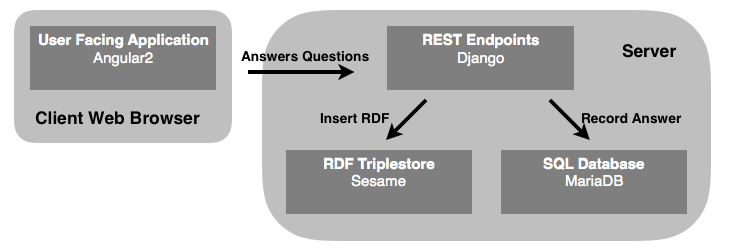
\includegraphics[width=1\textwidth]{pics/cafe_process.png}
  \caption{Components of the CAFE Application.}
  \label{cafe_process}
\end{figure}

The CAFE web application is a custom made site, built using Angular2 and Django, the source of which is available on Github (https://github.com/cafe-trauma/).
The questionnaire currently consists of just over 150 questions with various types of possible answers.
New questions are added to the site through an administrator interface by non-developers (figure of question admin interface).
Currently supported are yes/no, number field, check-box selection, and drop downs.
The answers to these questions have RDF representations also entered into the site through the administrator interface by a non-developer. (figure of rdf entry page)
These can range from a single RDF triple (figure of question 161) to a complex set of triples (figure of large rdf graph).
When a user answers a question in the positive, either yes on a yes/no or any selection on the other question types, the configured RDF for that question will be inserted into a triplestore on the server.
This RDF can also be generated later at anytime as the tool also records all answers to the questionnaire in the same relational database which holds the questions and potential triples.
From the users point of view the questionnaire does not differ in any way from a more typical questionnaire backed by a relational database.


\textcolor{red}{Also mention ability to share "original data" for the purpose of reproducibility and better transparency in science}

\section*{Results}
\textcolor{blue}{What do we actually want to say in the results section?}

\textcolor{red}{Maybe mention semantic survey here, or would that be better for future work?}

\section*{Discussion}
What we have set forth here is methodology for representing the answers to questionnaires directly into RDF.

\textcolor{red}{Advantages of semantic web, sharability/usability of generated data, question framing}

\section*{Future Work}
Another application we have built using this framework is the DIDEO(?) - evidence of potential drug-drug interaction classification tool.
In this tool trained users will enter properties from reported potential drug-drug interactions through a small number of questions.
These questions will generate RDF in the same way as the CAFE application.
After the questions are answered a logical reasoner is run over the generated RDF which can infer additional properties thus minimizing the number of questions the user will need to fill out.
In this example we are asking the user to answer 10 questions which using this inference can record the same amount of information that it would normally take many more questions to specify.

In both of these example applications the user is presented with a familiar looking survey presentation, but their answers will produce a semantically rich representation of what the questions are asking.  The generated data is immediately ready to be used with any existing RDF data or even translated back into a relational database format with all of the logical inferences intact.


\makeatletter
\renewcommand{\@biblabel}[1]{\hfill #1.}
\makeatother

\bibliographystyle{unsrt}
\begin{thebibliography}{1}
\setlength\itemsep{-0.1em}

\bibitem{ref1}
Pryor TA, Gardner RM, Clayton RD, Warner HR. The HELP system. J Med Sys. 1983;7:87-101.
\bibitem{ref2}
Gardner RM, Golubjatnikov OK, Laub RM, Jacobson JT, Evans RS. Computer-critiqued blood ordering using the HELP system. Comput Biomed Res 1990;23:514-28.

\end{thebibliography}

\end{document}
